\documentclass[11pt, a4paper, oneside]{scrartcl}
\usepackage[hidelinks]{hyperref}
\usepackage{polski}
\usepackage[utf8]{inputenc}

\usepackage{amssymb}
\usepackage{amsmath}
\usepackage[pdftex]{graphicx}
\usepackage[margin=2.0cm]{geometry}

\usepackage{algorithm2e}
\usepackage{algorithmic}
\usepackage{mathtools}
\usepackage{multirow}
\usepackage{pbox}
\usepackage{hyperref}
\usepackage{tikz}
\usepackage{tkz-euclide}
\usetkzobj{all} 
\usepackage{array}
\usepackage{float}

\author{Jadwiga Słowik \and Anna Bujak}

\title{Aplikacja \textit{Weather4Runners} \\ Raport}

\begin{document}
\maketitle

\section{Logika biznesowa}
Aplikacja wyświetla najlepsze propozycje godzinowe (filtrując prognozy pogody dla najbliższych $24$ godzin) oraz~najlepsze propozycje dniowe
(filtrując prognozy dla~najbliższych kilku dni). Optymalne warunki pogodowe są określane przez~użytkownika w~aplikacji.

Użytkownik może określić następujące parametry (niektóre z~nich może oznaczyć jako~nieistotne):
\begin{itemize}
	\item Temperatura powietrza
	\item Wilgotność powietrza
	\item Prędkość wiatru
	\item Zachmurzenie
	\item Opady
\end{itemize} 

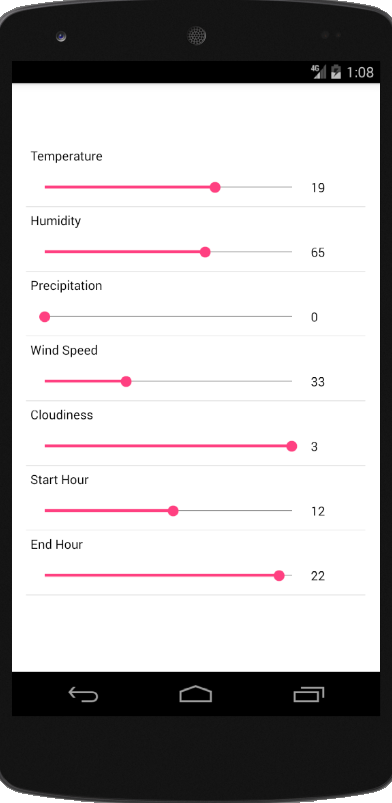
\includegraphics[scale=0.7]{screen_pref.png}
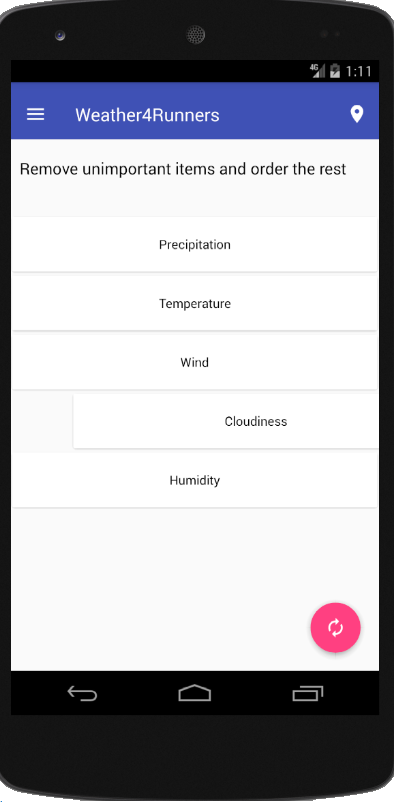
\includegraphics[scale=0.7]{screen_imp_cond.png}
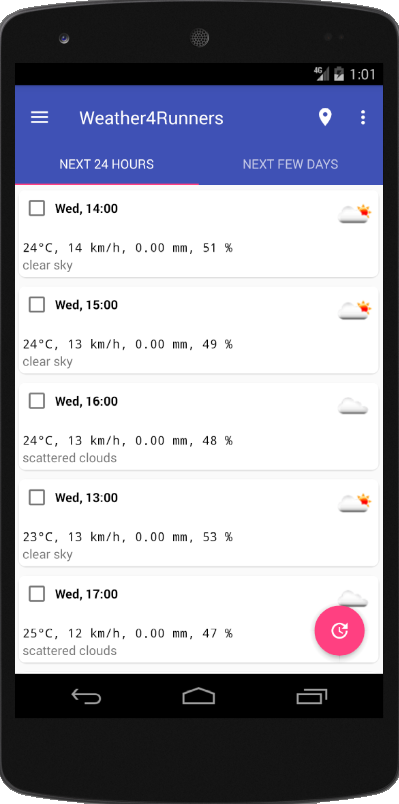
\includegraphics[scale=0.7]{screen_props.png}

Ponadto, użytkownik może określić, jaki~przedział godzinowy (godzina~początkowa, godzina~końcowa) go interesuje oraz~ile propozycji ma~być wyświetlane
na~ekranie.

Oprócz preferencji związanych z~filtrowaniem propozycji użytkownik może również określić, dla~jakiej lokalizacji prognoza pogody ma~być pobierana:

\begin{itemize}
	\item Aktualna lokalizacja
	\item Lokalizacja wpisana przez użytkownika (odpowiednie miasto i państwo)
\end{itemize}

\begin{center}
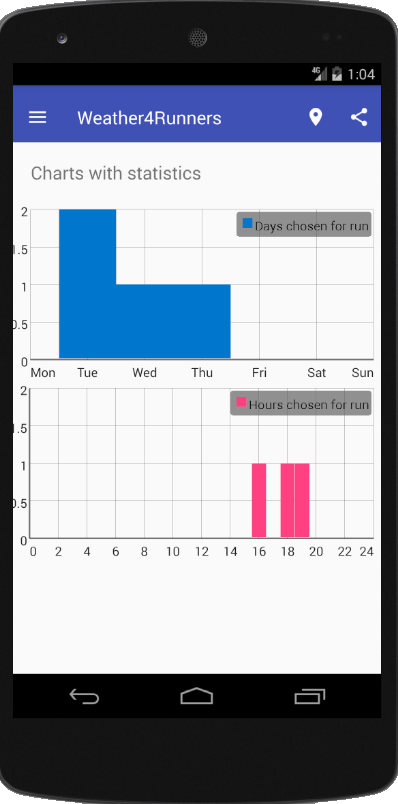
\includegraphics[scale=0.7]{screen_stats.png}
\end{center}

Otrzymawszy propozycje na ekranie, użytkownik ma możliwość wyboru (deklaracji) niektórych z~nich. Owe deklaracje są~odnotowywane
i~nanoszone na~odpowiednie wykresy, które~prezentują statystyki związane z~dotychczas dokonywanymi wyborami (jak~często dany dzień/dana godzina była wybierana).

\section{Architektura}
Aplikacja składa~się z~jednej aktywności, a~poszczególne ekrany zaimplementowane zostały za~pomocą fragmentów. Komunikacja pomiędzy komponentami
zachodzi za~pośrednictwem aktywności, która~implementuje odpowiednie interfejsy.

Dzięki temu, fragment ma ograniczoną wiedzę na~temat postaci aktywności i~posiada jedynie informacje konieczne do~jego poprawnego funkcjonowania
(tj. aktywność implementuje odpowiedni interfejs i~dzięki~temu można na~niej wywołać odpowiednią metodę).

\subsection{Pobieranie danych}
Pobierana jest prognoza pogody z~\textit{OpenAPI} (w naszym przypadku: \textit{OpenWeatherMap}). Dane są reprezentowane w~postaci \textit{JSON}
i~zawierają listę prognoz pogody dla~następnych pięciu dni co~trzy godziny.

Klasy służące do pobierania danych rozszerzają (i implementują jej metody) abstrakcyjną klasę \textit{JSONWeatherDownloader}. 
Obecnie mamy możliwość pobierania danych podając współrzędne geograficzne interesującego nas miejsca lub~podając jawnie miasto i~państwo.

Zarządzaniem obiektami związanymi z~pobieraniem danych zajmuje~się klasa \textit{WeatherDownloadersManager}, która~ma referencje
do~wszystkich obiektów-,,downloaderów'' i~pamięta, który jest obecnie ustawiony (\textbf{wzorzec projektowy Strategia}).

\subsection{Przetwarzanie danych}
\subsubsection{Ekstrakcja}
Przekształcamy dane \textit{JSON} na~obiekty reprezentujące dane pogodowe
(\textit{WeatherInfo}).  ,,Wyciąganie danych z~\textit{JSON}'' odbywa~się przy~pomocy implementacji klasy \textit{JSONOpenWeatherMapValuesExtractor}. Jej klasą bazową jest abstrakcyjna klasa \textit{JSONWeatherValuesExtractor}.

Dzięki takiej impelementacji
możliwa jest łatwa zmiana źródła danych --- wystarczy jedynie napisać nową klasę rozszerzającą klasę \textit{JSONWeatherValuesExtractor}.

\subsubsection{Przybliżanie wartości}
Obecne API zapewnia nam prognozy pogody co~trzy godziny. Wobec tego, musimy przekształcić w~taki sposób dane pogodowe,
aby~mieć prognozy co~jedną godzinę.

Istnieje wiele sposobów przybliżania wartości. Jednym z~nich jest interpolacja liniowa. Warto zaznaczyć, że~obecna implementacja
pozwala na~łatwe rozszerzenie/zmianę opisywanego kroku algorytmu. Została utworzona abstrakcyjna klasa \textit{WeatherInfosApproximator},
która dostarcza abstrakcyjną metodę odpowiedzialną za~obliczanie wartości pośrednich (skrajne wartości pogodowe oraz~liczbę wartości do~wygenerowania
określamy w~konstruktorze).

Obecnie, została zaimplementowana klasa do~interpolacji liniowej, która~rozszerza powyżej przedstawionę klasę.

\subsubsection{Połączenie pobierania i uśredniania danych}
Główną klasą odpowiedzialną za~przetwarzanie i pobieranie danych jest \textit{JSONTransformator}. Jej dwa główne pola są związane z~parsowaniem
(ekstrakcją danych) oraz~przybliżaniem wartości pośrednich.

Jest ona tworzona przy~pomocy \textbf{wzorca projektowego Budowniczy} (w~naszym
przypadku jest to klasa \textit{JSONTransformatorBuilder}). Dzięki temu, nasza architektura jest modularna i~możemy podmienić algorytm
związany z~przybliżaniem niezależnie od~algorytmu parsowania.

\subsubsection{Filtrowanie danych}
Kolejność prezentowanych użytkownikowi propozycji jest zależna od~jego preferencji dotyczących warunków pogodowych. Dla~każdej prognozy pogody
obliczamy wartość określająca ,,odległość od~optymalnych warunków pogodowych'' (im~większa wartość, tym~gorsza propozycja).
Następnie, sortujemy dane propozycje. 

\subsection{Zapis danych}
Dane (pobrane prognozy pogody, preferencje dt. warunków pogodowych użykownika, deklaracje) są~składowane w~bazie danych \textit{SQLite},
natomiast preferencje związane z~liczbą propozycji do~wyświetlenia oraz~wybraną lokalizacją przy~pomocy \textit{SharedPreferences}.

\subsection{Wykresy}
Wykresy dotyczące wybranych propozycji zostały utworzony przy~pomocy biblioteki \textit{GraphView}.

\end{document}